\documentclass[a4paper, 12pt]{article}
\usepackage{titling}
\usepackage{array}
\usepackage{booktabs}
\usepackage{enumitem}
\usepackage{graphicx}
\usepackage{hyperref}
\usepackage{amssymb}
\setlength{\heavyrulewidth}{1.5pt}
\setlength{\abovetopsep}{4pt}
\setlength{\parindent}{0pt}
\graphicspath{{.}}

\usepackage[margin=1in]{geometry}

% Must be after geometry
\usepackage{fancyhdr}
\pagestyle{fancy}
\fancyhf{}
\rhead{NN Homework 1}
\lhead{P.Lukin, I. Vishniakou, E. Ovchinnikova}
\cfoot{\thepage}

\setlength{\droptitle}{-5em}

\title{Neural Networks  \\
				- Homework 1 -}
\author{Petr Lukin, Ivan Vishniakou, Evgeniya Ovchinnikova}
\date{Lecture date: 26 September 2016}

\begin{document}

\maketitle

\section{Mind map}
Neural network (NN) is a parallel distributed system consisted of computing cells ("neurons") that is capable of storing and using experimental knowledge to model a brain in processes of certain tasks performance.

\begin{figure}[h]
  \centering
  \caption{S. Haykin, Neural Networks, chapter 1. Mind map (a zoomed version of the map is attached as NN.png file).\label{fig:mindMap}}
  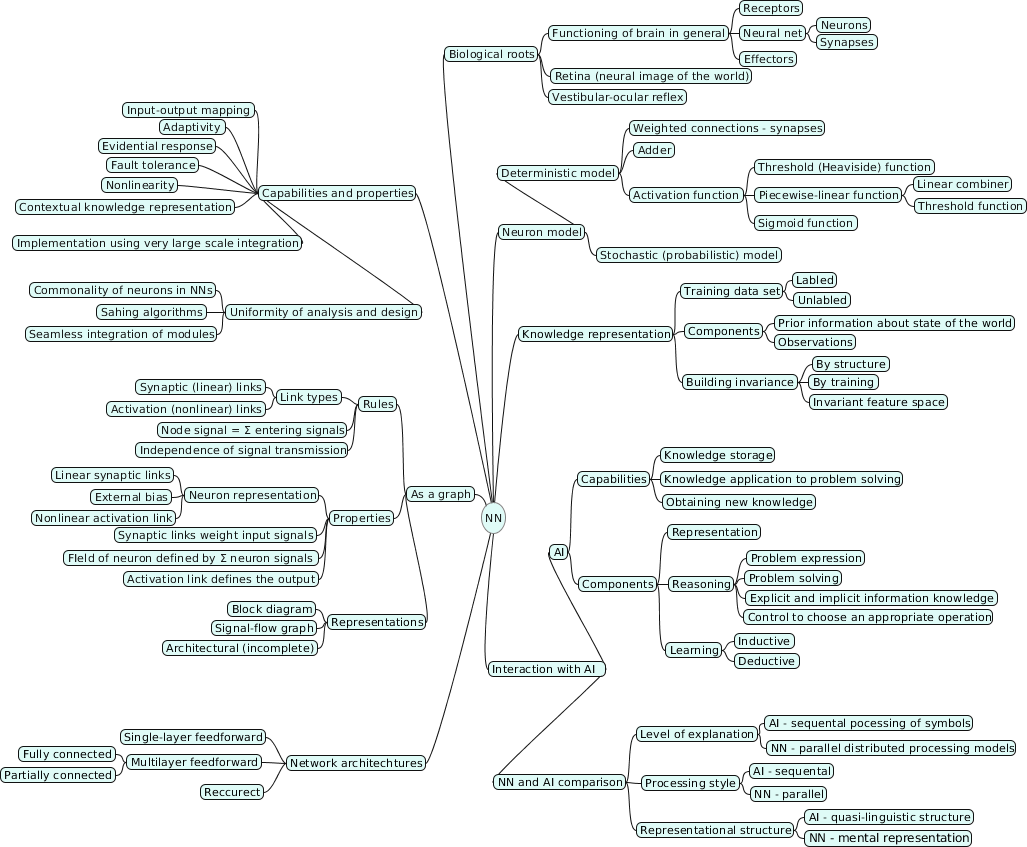
\includegraphics[width=1.0\textwidth]{NN}
\end{figure}

\section{Exercises}

\subsection{Exercise 1.1}

$\phi(v) = \frac{1}{1 + exp(-av)}$\\

Show that $\frac{d\phi(v)}{dv} = a\phi(v)[1 - \phi(v)]$. What is the value of this derivative at the origin?\\

Solution:\\

$\frac{d\phi(v)}{dv} = \frac{d((1 + exp(-av))^{-1})}{dv} = -\frac{-a\cdot exp(-av)}{(1 + exp(-av))^2} = \frac{a(exp(-av) + 1 -1)}{(1 + exp(-av))^2} = \frac{a}{(1 + exp(-av))} (1 - \frac{1}{(1 + exp(-av))}) = a\phi(v)[1 - \phi(v)]$\\

$\frac{a}{(1 + exp(-a\cdot 0))} (1 - \frac{1}{(1 + exp(-a\cdot 0))}) = \frac{a}{(1 + 1)} (1 - \frac{1}{(1 + 1)}) = \frac{1}{4}$


\subsection{Exercise 1.3}

$\phi(v) = \frac{v}{\sqrt{1+v^2}}$\\


Show that $\frac{d\phi(v)}{dv} = \frac{\phi(v)^3}{v^3}$. What is the value of this derivative at the origin?\\

Solution:\\

$\frac{\phi(v)^3}{v^3} =\frac{1}{(\sqrt{1+v^2})^3} $\\

$\frac{d\phi(v)}{dv} = \frac{\sqrt{1+v^2}-v 0.5(\sqrt{1+v^2})^{-1}2v}{(\sqrt{1+v^2})^2} = \frac{\sqrt{1+v^2}-v^2 (\sqrt{1+v^2})^{-1}}{(\sqrt{1+v^2})^2} = \frac{1+v^2-v^2}{(\sqrt{1+v^2})^3}=\frac{1}{(\sqrt{1+v^2})^3} $\\

$\phi(0) = \frac{0}{\sqrt{1+0^2}} = 0$\\


\subsection{Exercise 1.12}

A fully connected feedforward netwok has 10 source nodes, 2 hidden layers, one with 4 neurons and the other with 3 neurons, and a single output neuron. Construct an architectural graph of this network.

\includegraphics[scale=0.2]{112.png}


\subsection{Exercise 1.13}
\subsubsection{a)}
Figure shows the signal flow graph of a 2-2-2-1 feedforward network. The function $\phi()$ denotes a logistic function. Write the input - output mapping defined by this network.

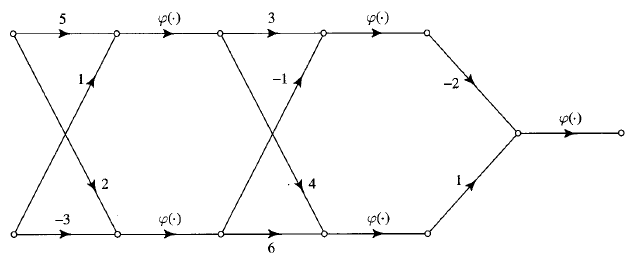
\includegraphics[scale=0.7]{113.png}

Solution:\\

Let input values be $x_1,x_2$. Lets propagate this values through all hidden layers:

$v_{1,1} = \phi(5x_1+x_2)$ \\

$v_{1,2} = \phi(2x_1-3x_2)$ \\

$v_{2,1} = \phi(3v_{1,1}-v_{1,2})$ \\

$v_{2,2} = \phi(4v_{1,1}+6v_{1,2})$ \\

$v = \phi(-2v_{2,1}+v_{2,2})$ \\

Lets unfold the previous equations:
\\

$v = \phi((\phi(3(\phi(5x_1+x_2))-(\phi(2x_1-3x_2))))+(\phi(4(\phi(5x_1+x_2))+6(\phi(2x_1-3x_2)))))$

\subsubsection{b)}
Suppose that the output neuron in the signal flow graph operates in its linear region. Write the input-output mapping defined by this new network.

If the output neuron operates in its linear region sigmoid function can be substituted with linear function. Thus, sigmoid function will nt be applied in the end:
\\

$v = \phi(3(\phi(5x_1+x_2))-(\phi(2x_1-3x_2))))+\phi(4(\phi(5x_1+x_2))+6(\phi(2x_1-3x_2))$




\end{document}
